\documentclass[a4paper,titlepage,onecolumn,twoside,12pt]{article}
\usepackage{ucs} %unix-windows-compatible
\usepackage[utf8x]{inputenc} %unix-windows-compatible
\usepackage[german,ngerman, english]{babel} %automatic text in german
\usepackage{verbatim} %for long comments
\usepackage{latexsym} %for symbol font
\usepackage{color,graphicx} %for inserting color and graphics
\usepackage{tabularx}
\usepackage[T1]{fontenc}
\usepackage{ae}
\usepackage{geometry} %for setting the margins
\setcounter{secnumdepth}{4} %numbering of the subsubsections
\setlength{\parindent}{0pt} %no indentation between paragraphs
\setlength{\parskip}{4pt} %space between paragraphs
\usepackage[margin=10pt,font=small,labelfont=bf,]{caption} [2003/12/20]
\frenchspacing % erzeugt ein wenig mehr Platz hinter einem "." so wie im Dt. ueblich
% define the fancy header:
\usepackage{fancyhdr} 
\fancyhf{} % delete current header and footer
\fancyhead[LO]{\bfseries\rightmark}
\fancyhead[RE]{\bfseries\leftmark}%for twoside-option
\renewcommand{\headrulewidth}{0.5pt}
\renewcommand{\footrulewidth}{0pt}
\addtolength{\headheight}{2.5pt} % space for the rule
\fancypagestyle{plain}{%
	\fancyhead{} % get rid of headers on plain pages
	\renewcommand{\headrulewidth}{0pt} % and the line
}
\pagestyle{fancy}
\cfoot{\thepage}
\usepackage[pdfpagelabels=true
%,backref %references in Literatur-Verz.
, hyperfigures
, bookmarksnumbered
, naturalnames
, plainpages=false
]{hyperref}
\definecolor{darkblue}{rgb}{0,0,.4}
\definecolor{darkred}{rgb}{.4,0,0}
\definecolor{darkgreen}{rgb}{0,0.4,0}
\hypersetup{breaklinks, colorlinks, linkcolor=darkblue, menucolor=darkblue, pagecolor=darkblue, urlcolor=darkblue, citecolor=darkgreen}
\usepackage[figure]{hypcap} % a link jumps and focus on the picture and not on the caption
%

%
%%%%%%%%%%%%%%%%%%%%%%%%%%%%%%%%TITEL%%%%%%%%%%%%%%%%%%%%%%%%%%%%%%%%%%
% define the title:
\author{\Large%
NAME\\{\normalsize Matr.-Nr. %
NUMMER} \\}
\title{
\vspace{-13em}
\centering
\begin{figure*}[!hb]
  \begin{minipage}{1\textwidth}
\hspace*{-.06\linewidth}
  \begin{minipage}{.13\linewidth}
    
\includegraphics[width=1.0\linewidth]{tu_logo_3d_rot}
  \end{minipage}
	\quad\quad
  \begin{minipage}{.67\linewidth} 
Fachgebiet Software and Embedded Systems Engineering\\
Fakult\"at IV Elektrotechnik und Informatik\\
Technische Universit\"at Berlin
  \end{minipage}
%	
  \begin{minipage}{.19\linewidth}
    
\includegraphics[width=1.0\linewidth]{logo}    
  \end{minipage}  
  \caption*{}
  \end{minipage}  
\end{figure*}
\vspace{8em}
{\huge\textbf{%
%
Zentrale vs. Dezentrale Adaptierungsplanung in Multidrohne-Szenarien
}}\\ \vspace{1.7cm}{\LARGE{\bfseries Bachelorarbeit}\\\vspace{0.6cm}
}}
\date{%
DATUM \\
\vspace{9em}
\large
\textbf{Betreuer:} \\
\vspace{1em}
Prof. Dr. Sabine Glesner\\
- WiMi -\\
- ggf. WEITERER WiMi -
}

%
\begin{document}
\newpage\thispagestyle{empty}\pagenumbering{alph}
\enlargethispage{20\baselineskip}
\oddsidemargin5mm
% generates the title: 
\addtolength{\textwidth}{3em}
%
\maketitle
%
\addtolength{\textwidth}{-3em}
%
%--------- new section:--------------------------------
\newpage\thispagestyle{empty}
\cleardoublepage
\evensidemargin-6mm
\oddsidemargin6mm
\newpage\thispagestyle{empty}\section*{Eidesstattliche Erkl\"arung}
\vspace{2.5cm} Hiermit erkläre ich, dass ich die vorliegende Arbeit selbstst\"andig und eigenh\"andig sowie ohne unerlaubte fremde Hilfe und 
ausschlie{\ss}lich unter Verwendung der aufgef\"uhrten Quellen und Hilfsmittel angefertigt habe. \\
\\ \vspace{1.2cm}\\
\line(1,0){250} \\
%-------------------------------------------------------------%
\\
$~{}~{}~{}~{}~{}~{}$Berlin, den DATUM 
%--------- new section:--------------------------------
%\newpage\thispagestyle{empty}
%\cleardoublepage
%\newpage\thispagestyle{empty}\section*{Danksagung}
%
\newpage\thispagestyle{empty}
\cleardoublepage
\selectlanguage{german}
\newpage\thispagestyle{empty}\section*{Zusammenfassung}
{\small DEUTSCHES ABSTRACT}
\selectlanguage{english}
\section*{Abstract}
{\small ENGLISCHES ABSTRACT}

%REIHENFOLGE KANN AUCH GETAUSCHT WERDEN

%%%%%%%%%%%%%%%%%%%%%%%%%%%%%%CONTENT%%%%%%%%%%%%%%%%%%%%%%%%%%%%%%%%
\selectlanguage{german}
\newpage\thispagestyle{empty}
\cleardoublepage
\newpage\pagenumbering{roman}\thispagestyle{plain}
% insert the table of contents:
\pdfbookmark[1]{Inhaltsverzeichnis}{Inhalt}
\tableofcontents\thispagestyle{plain}
%
%%%%%%%%%%%%%%%%%%%%%%%%%%%%%%FIRST PAGE%%%%%%%%%%%%%%%%%%%%%%%%%%%%
\newpage\thispagestyle{plain}
\hypersetup{breaklinks, linkcolor=darkred}
\cleardoublepage
\newpage\newcounter{1}\thispagestyle{plain}\pagenumbering{arabic}
\section{Einleitung}
\label{sec:einleitung}
%
%
%
%
HIER BEGINNT DIE ARBEIT
%
%
%
%
%Gliederung
\subsection{Motivation}
\label{subsec:motivation}
Koordination bedeutet das aufeinander Abstimmen  der verschiedenen Komponenten, die ein Kollektiv ausmachen. Als entscheidendes Ziel eines Selbst-adaptiven 
Systems kann auch die Koordination der einzelnen Komponenten als Teil der Anpassung betrachtet werden. 
Um mit dem unsicheren und statisch unvorhergesehenen Umgebungsverhalten komplexer Systeme fertig zu werden, hat die Selbstanpassungsfähigkeit breite 
Akzeptanz gefunden.
Als Beispiel betrachten wir einen Lieferservice, der aus selbst-adaptiven Drohnen besteht.
 
Selbst-adaptive Systeme verfügen über die Fähigkeit, sich an Änderungen in ihrer Ausführungsumgebung und inneren Dynamik zu adaptieren, wie beispielsweise 
Reaktion auf Ausfall, Variabilität der verfügbaren Ressourcen oder sich ändernde Benutzerprioritäten, um weiterhin ihr Ziel zu erreichen [1]. Das 
ermöglicht den Drohnen, z.B. ihre Flughöhe anzupassen, wenn sie einen neuen Bereich betreten, in dem andere Regelungen gelten oder zum Akkusparmodus zu 
wechseln, wenn ihr Akkustand einen bestimmten Grenzwert erreicht. Rückkopplungsregelkreise wurden als entscheidende Elemente in der Realisierung der 
Adaptierung von Softwaresystemen identifiziert [1]. Zu diesem Zweck benutzen wir IBMs MAPE-K Schleife. Diese Schleife besteht aus 4 Phasen, nämlich 
“Monitor”, “Analyse”, “Plan” und “Execution”, die zusammen eine statische Adaption unseres Systems ausführen.
\subsection{Problemstellung}
\label{subsec:problem}
Die Ausgangslage ist ein Szenario, in dem eine Menge von selbst-adaptiven Drohnen einen Lieferservice in einer sich ändernden Umgebung vornehmen muss,
wobei jede Drohne über ein voneinander unabhängiges System verfügt. Hierbei entsteht das Problem, dass Adaptionen mehrere Drohnen betreffen können oder die 
Mitarbeit einer anderen Drohne erfordert. Bei einem Ausweichmanöver zur Kollisionsvermeidung sollte beispielsweise die Flughöhe so angepasst werden, dass 
die Anpassung beider beteiligter Drohnen nicht in die selbe Richtung erfolgt. Die Mitarbeit einer anderen Drohne ist zum Beispiel erforderlich, wenn eine 
Drohne aufgrund niedrigen Batteriestands ihr Transportgewicht reduzieren muss um sicher bis zur Ladestation zu kommen. Hier sollte eine andere Drohne 
Pakete übernehmen können. Lokale Adaptionen stoßen hier an ihre Grenzen. 


Im nächsten Absatz stellen wir unsere Lösungen dar, um diese Probleme zu beheben.
\subsection{Ziel und Lösungsansatz}
\label{subsec:ziel}
Wenn die Systeme groß, komplex und heterogen sind, reicht eine einzelne MAPE-K Schleife möglicherweise nicht aus, um die Adaptierung auszuführen. In 
solchen Fällen können mehrere MAPE-Schleifen verwendet werden, die verschiedene Teile des Systems verwalten [1] und Informationen austauschen. Im Bereich 
der Koordination von mehreren voneinander unabhängigen Systemen stehen viele Design-Möglichkeiten zur Verfügung. Diese sind grundsätzlich zwei: der (a) 
zentrale und der (b) dezentrale (oder verteilte) Ansatz. (a) könnte zum Beispiel umgesetzt werden durch eine hierarchische Anordnung der MAPE-K Loops, 
wobei jede Ebene der Hierarchie Instanzen von allen vier MAPE-Komponenten enthält [1]. Für (b) liegen mehrere Schemata vor, die verschiedene Ansätze durch 
Zentralisierung und Dezentralisierung der Funktionen der Selbstadaptation auf unterschiedliche Weisen [1] darstellen. 



Nun werden die Ziele dieser Arbeit definiert. Erstens möchten wir eine Anwendung zur “Multi-Drohnen Kollisionsvermeidung” entwickeln. Dazu erstellen wir 
einen Konsens über Flugkorridore in verschiedenen Höhen. Die Korridore müssen sich an die individuellen Einschränkungen jeder Drohne halten. Zweitens, wird 
auch eine Anwendung zur “Multi-Drohnen Paket Optimierung” entwickelt. Diese Anwendung ermöglicht, dass die Drohnen Pakete von anderen Drohnen übernehmen 
können, wenn deren Akkustand niedrig ist.

 
Zu diesem Zweck  ist ein Informationsaustausch zwischen den Drohnen erforderlich. Wie oben erklärt, gibt es hierfür zwei Vorgehensweisen: der zentrale und 
der dezentrale Ansatz. Um den ersten Ansatz auszuführen, benutzen wir eine hierarchische Anordnung der MAPE-K Schleifen. Um den zweiten Ansatz vorzunehmen, 
benutzen wir Dezentralisierungsvorlagen in [1] präsentiert. Schließlich nehmen wir eine Vergleichung beider Ansätzen miteinander vor.

 
Darüber hinaus realisieren wir eine Implementation der zentralen und dezentralen Systemen für die Anwendung zur “Multi-Drohnen Kollisionsvermeidung” , 
wobei c++ Programmiersprache benutzt wird und SystemC Kanäle für die Kommunikation verantwortlich sind. Als ein wünschenswertes Ziel, implementieren wir 
auch die Anwendung zur “Multi-Drohnen Paket Optimierung”. Falls es die Zeit nicht erlaubt, erklären wir die Vorgehensweise, wie man das implementieren 
könnte.

\subsection{Hintergrund des MAPE-Ks}
\label{subsec:hintergrund}
\subsection{Verwandte Arbeiten} %ggf. eigene Section
\label{subsec:verwandte}

\section{Drohnenanordnungsmethode}
\label{sec:drohnenanordnungs}
Zuallererst stellen wir unsere Drohnenanordnungsmethode vor. Es handelt sich um eine Methode, deren Aufgabe es ist, einen Plan zur Anpassung der Flughöhe 
der Drohnen durchzuführen und dabei enge Flugbähne und ggf. Kollisionen zu vermeiden. Im Gegensatz zur Annäherung zweier Luftfahrzeuge mit 
Kollisionsgefahr, wobei meistens Ausweichregeln zwischen Luftfahrzeugen zum Tragen kommen, stellt unsere Drohnenanordnungsmethode eine vorbeugende Maßnahme   
dar, die den Luftraum aufteilt. 

Beispiele von Ausweichmanöver\footnote{https://de.wikipedia.org} bei Kollisionsgefahr können wir in den Abbiludungen 
\ref{fig:encounter}, \ref{fig:cross} und \ref{fig:overtaking} sehen. Eine Annäherung mit Kollisionsgefahr ist tatsächlich eine Situation, die für 
Verkehrsflugzeuge extrem selten stattfindet, denn dafür werden TCAS's (Traffic Alert and Collision Avoidance System) benutzt, die spezifische
"`Schutzzonen"' um die eigenen Flugzeuge definiert und dazu beiträgt, zu nahe beieinander liegende Flugbahnen und damit das Risiko einer Annäherung mit 
Kollisionsgefahr zu vermeiden.

Die Drohnenanordnungsmethode wird innerhalb einer Gruppe von Drohnen aufgerufen und ausgeführt, die zu nahe beieinander liegen. Späterhin bei den 	
Abschnitten \ref{sec:zentral} und \ref{sec:dezentral} betrachten wir zwei verschiedene Wege, durch die wir Gruppen von Drohnen bilden, die einander nahe 
stehen. Im Moment erklären wir jedoch, wie die Methode innerhalb eine Gruppe funktioniert.


\begin{figure}
\centering

\includegraphics[width=0.3\textwidth]{120px-Encounter_rule}
\caption{Einander entgegenkommende Luftfahrzeuge haben stets nach rechts auszuweichen.}
\label{fig:encounter}
\end{figure}

\begin{figure}
\centering
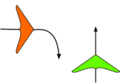
\includegraphics[width=0.3\textwidth]{120px-Crossing_rule}
\caption{Von links kommende Luftfahrzeuge sind ausweichpflichtig.}
\label{fig:cross}
\end{figure}


\begin{figure}
\centering
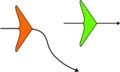
\includegraphics[width=0.3\textwidth]{120px-Overtaking_rule}
\caption{Überholende Luftfahrzeuge haben rechts am Überholten vorbeizufliegen.}
\label{fig:overtaking}
\end{figure}


\subsection{Funktionssweise}
\label{subsec:funktionssweise}
Nun erklären wir die Funktionsweise unserer Methode. Eine Schleife durchläuft alle Korridore von oben nach unten. Bei jedem Korridor überprüfen wir zunächst, ob dieser überbelegt ist bzw. er hat mehr als eine Drohne. Um das zu bestimmen, steht es uns bei der Planning-Phase zur Verfügung, einen Vorgang zur Erkennung des Korridors, in dem jede Drohne zu diesem Zeitpunkt fliegt. Eine vollständige Erklärung zur Methode finden wir im Abbildung \ref{fig:drohnenanordnung}.

Wenn es mehr als eine Drohne in einem Flugkorridor gibt, müssen die überschüssige Drohnen also in andere Korridore fliegen, bis die Überbelegung gelöst ist. Um zu entscheiden, welche Drohne den Korridor an der ersten Stelle verlassen soll, verwenden wir ein Gewichtskriterium. Dieses lautet wie folgt: "`Die leichteste Drohne im überbelegtem Korridor muss sich an der ersten Stelle bewegen"'. Da die Drohnen einen Lieferservice ausmachen, trägt jede ein unterschiedliches Gewicht. Die Verwendung des Gewichts als Kriterium bietet uns eine hohe Zeit- und Energieeffizienz, denn eine leichtere Drohne erreicht ihr neues Flugziel schneller, wobei sie auch weniger Energie verbraucht.

Zur Veranschaulichung unserer Methode verwenden wir ein Beispiel. In der Abbildung \ref{fig:drohnenanordnungs_beispiel} sehen wir, wie die Methode Schritt für Schritt funktioniert.

\begin{figure}
\centering
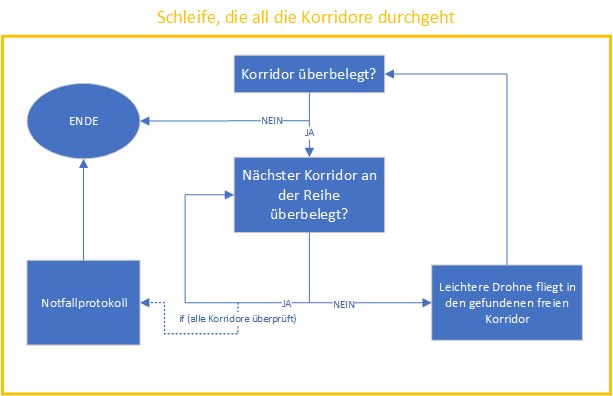
\includegraphics[width = 0.7\textwidth]{Drohnenanordnungsmethode}
\caption{Vorgehensweise der Drohnenanordnungsmethode}
\label{fig:drohnenanordnung}
\end{figure}

\begin{figure}
\centering
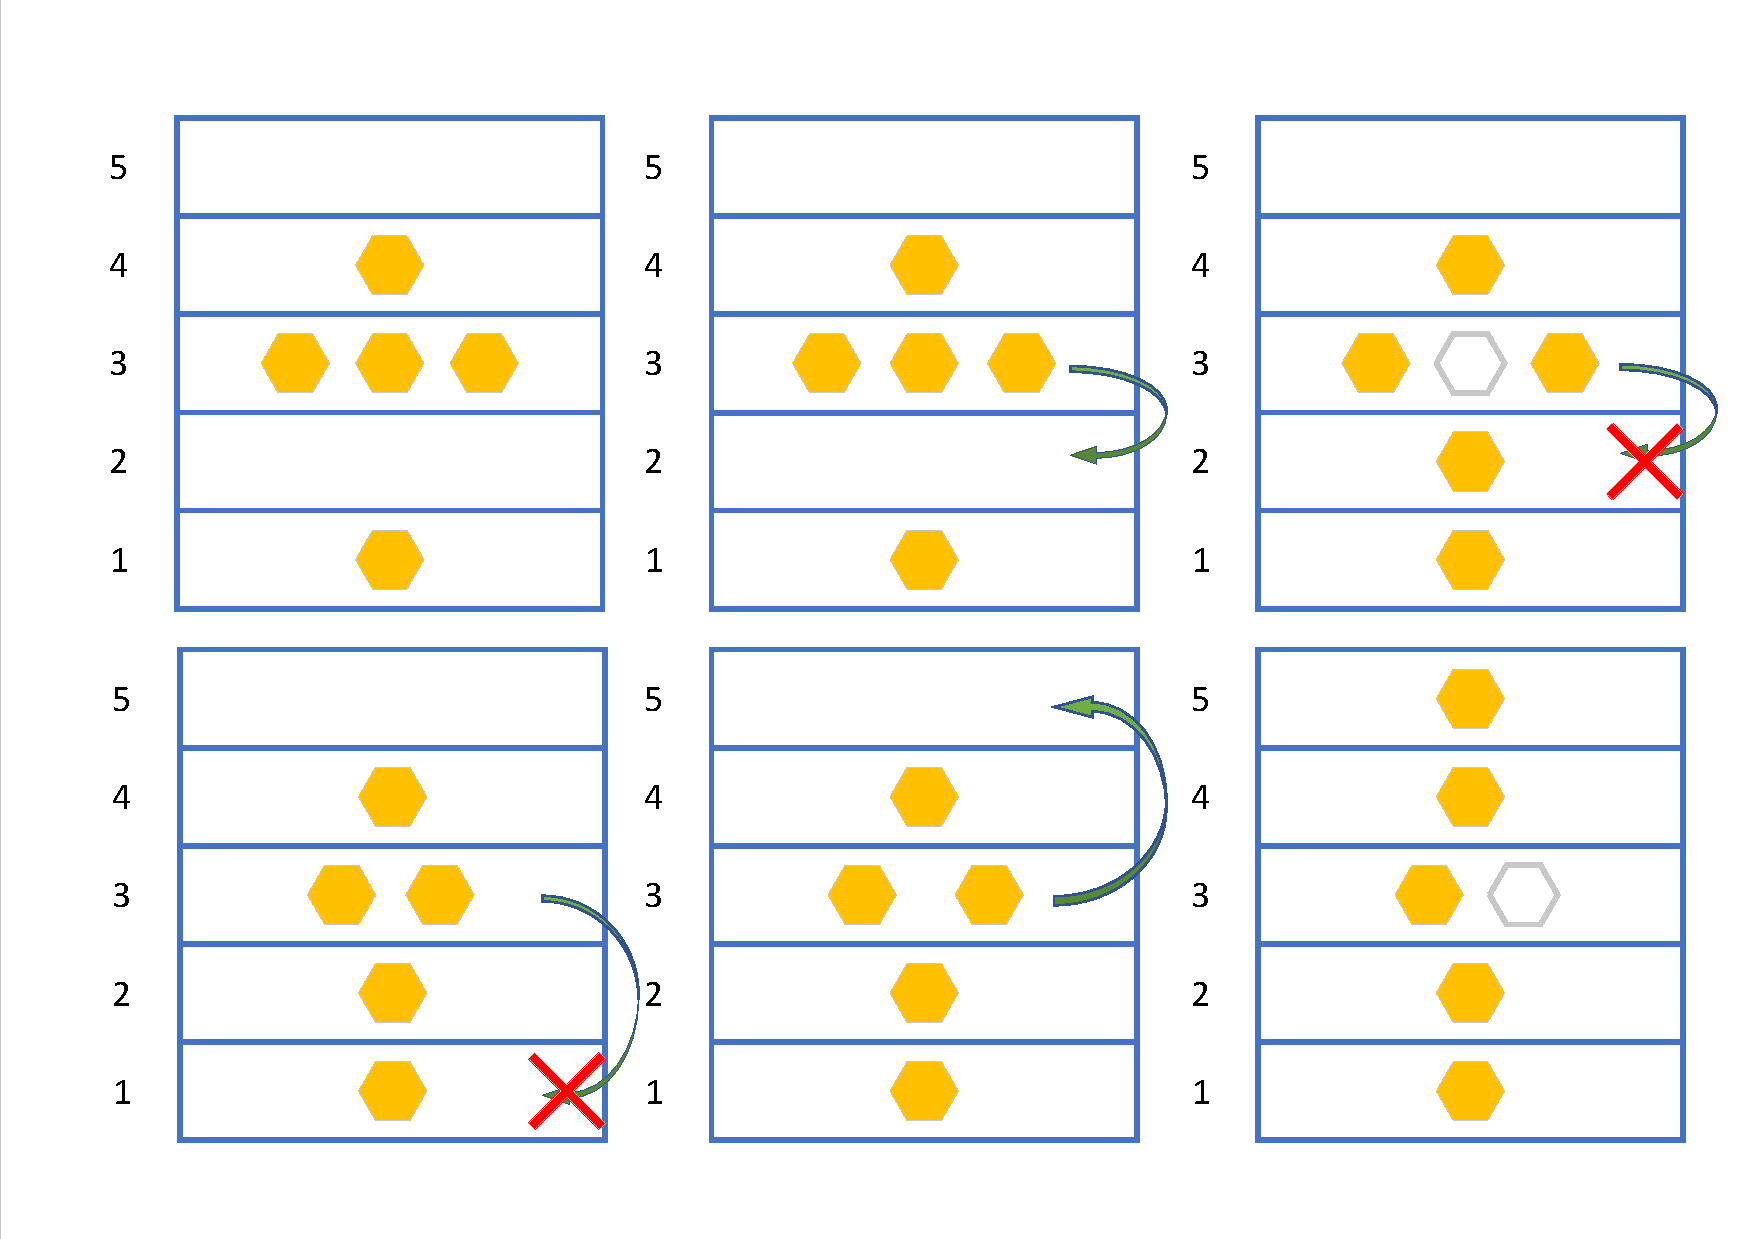
\includegraphics[width = 0.6\textwidth]{Drohnenanordnungsmethode_Beispiel}
\caption{Illustratives Beispiel der Drohnenanordnungsmethode}
\label{fig:drohnenanordnungs_beispiel}
\end{figure}

\subsection{Dimensionen}
\label{subsec:dimensionen}

Im Folgenden stellen wir eine erste Annäherung an die Dimensionen dieser Flugkorridoren in der realen Welt vor. Unter Berücksichtigung einer Dicke der Drohnen von ungefähr 0,5 Metern (einschließlich des Paketes) schlagen wir vor, Korridore von 6 Metern einzurichten. Dies bietet den Drohnen einen angemessenen Sicherheitsbereich und ermöglicht Kreuzungen ohne Störungen aufgrund Luftströmungen. In der Regel stellt sich eine Drohne in der Mitte ihres Korridors.

\begin{figure}
\centering
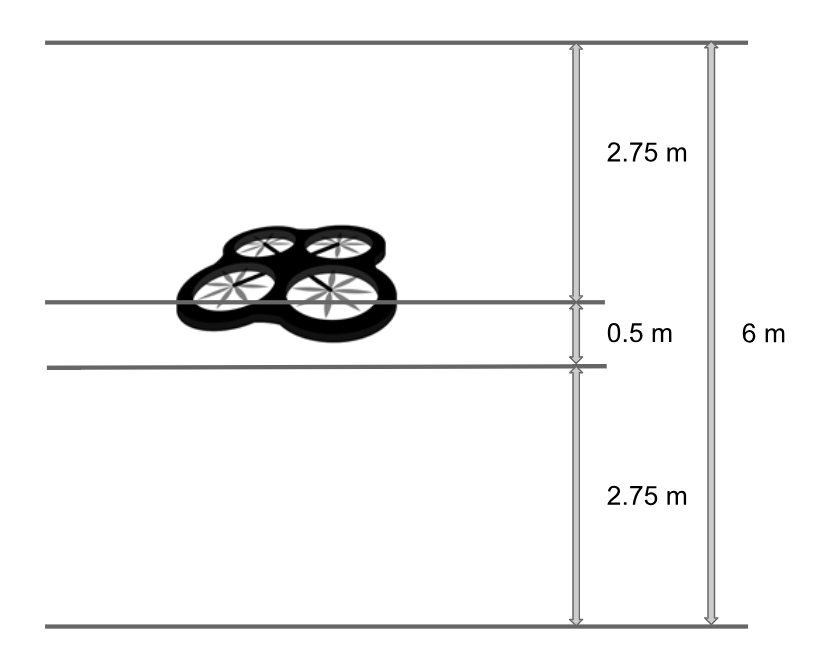
\includegraphics[width = 0.4\textwidth]{Flugkorridore_Dimensionen}
\caption{Dimensionen des Flugkorridors}
\label{fig:drohnenanordnungs_beispiel}
\end{figure}

%Kurze Zusammenfassung dessen, worüber wir in diesem Abschnitt gesprochen haben
In diesem Abschnitt haben wir sowohl die Flugkorridore als auch unsere Dronenanordnungsmethode vorgestellt. Als nächstes sprechen wir über den ersten Ansatz bei der Adaptierungsplanung: der zentraler Ansatz.

\section{Kollisionsvermeidung: Zentraler Ansatz}
\label{sec:zentral}

Wie in Abschnitt \ref{subsec:hintergrund} erklärt, ein prominenter Ansatz zum Organisieren einer Regelschleife in selbstadaptiven Systemen besteht aus vier Komponenten, die für die Hauptfunktionen der Selbstanpassung verantwortlich sind: Überwachen, Analysieren, Planen und Ausführen, häufig als MAPE-Schleife bezeichnet \cite{Prager1961}. Bei einem zentralen Ansatz verwenden wir ausschließich eine MAPE-K Schleife für die Koordination unseres ganzen System. Das heißt, all die verschiedenen Gruppen von Drohnen, in denen eine Drohnenanordnungsmethode (siehe Abschnitt \ref{sec:drohnenanordnungs}) abgerufen wird, müssen von einer einzigen, allgemeinen Schleife geregelt werden. Der erste Schritt zu diesem Zweck ist die Festlegung, nach welchem Kriterien wir lokale Gruppe von Drohnen definieren, wo Drohnen zu nahe voneinander stehen.

\subsection{Gruppenerkennung}
\label{sec:gruppenerkennung}

\subsubsection{Grundlagen}
\label{subsubsec:grundlagen}

Ein einfaches Beispiel für eine Gruppe von zu nahe beieinander stehenden Drohnen ist derjenige, wo jede Drohne zu nahe von all den Rest ist. Die Abbildung \ref{fig:gruppenerkennung_beispiele1} stellt ein Beispiel für diesen Fall dar. In der Praxis gibt es aber kompliziertere Fälle. Abbildung \ref{fig:gruppenerkennung_beispiele2} veranschaulicht einen Fall, wo drei Drohnen eine "`Kettenanordnung"' erzeugen, d.h. jede Drohne befindet sich ausschließlich der nächsten Drohne in der Kette zu nahe. Solche Ketten, die auch über vielfache Zweige verfügen können, werden auch als einzelne Gruppe betrachtet.



\begin{figure}
\centering
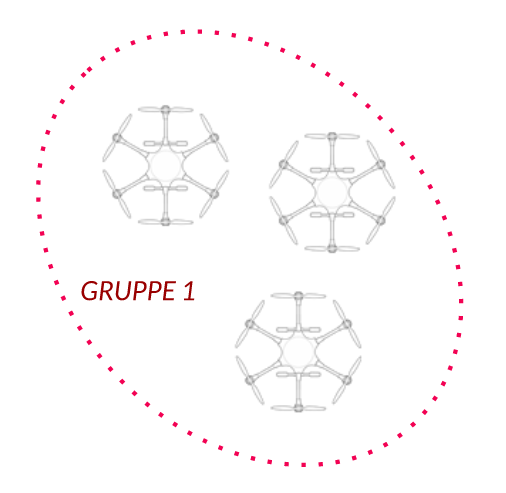
\includegraphics[width = 0.4\textwidth]{Gruppenerkennung_beispiele1}
\caption{Jede Drohne steht zu nahe von all den Rest}
\label{fig:gruppenerkennung_beispiele1}
\end{figure}

\begin{figure}
\centering
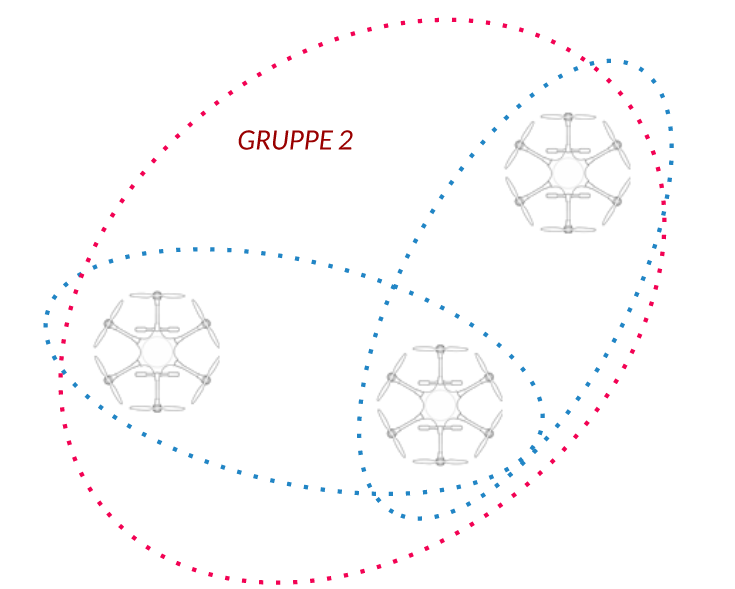
\includegraphics[width = 0.4\textwidth]{Gruppenerkennung_beispiele2}
\caption{Kettenanordnung}
\label{fig:gruppenerkennung_beispiele2}
\end{figure}

\section{Kollisionsvermeidung: Dezentraler Ansatz}
\label{sec:dezentral}
\section{Evaluierung}
\label{sec:evaluierung}
%Experimente, Tests, ..
\section{Zukünftige Arbeit}
\label{sec:zukünftige}
\section{Fazit}
\label{sec:fazit}
%Zusammenfassung und Ausblick

%
%

%%%%%%%%%%%%%%%%%%%%%%%%%%%%%%BIBLIOGRAPHY%%%%%%%%%%%%%%%%%%%%%%%%%%%%
\cleardoublepage
\newpage\thispagestyle{plain}\phantomsection
\addcontentsline{toc}{section}{\bibname}
\bibliographystyle{plain} %din-norm for citations feb 06
\bibliography{mylib}{}
\nocite{*}

%
\end{document}